\section{Strength and Weakness}

\subsection{Strength}

\begin{itemize}
\item We analyze the problem based on thermodynamic formulas and laws, so that the model we established is of great validity.

\item Our model is fairly robust due to our careful corrections in consideration of real-life situations and detailed sensitivity analysis.

\item Via Fluent software, we simulate the time field of different areas throughout the bathtub. The outcome is vivid for us to understand the changing process.

\item We come up with various criteria to compare different situations, like water consumption and the time of adding hot water. Hence an overall comparison can be made according to these criteria.

\item Besides common factors, we still consider other factors, such as evaporation and radiation heat transfer. The evaporation turns out to be the main reason of heat loss, which corresponds with other scientist’s experimental outcome.
\end{itemize}

\subsection{Weakness}

\begin{itemize}
\item Having knowing the range of some parameters from others’ essays, we choose a value from them to apply in our model. Those values may not be reasonable in reality.

\item Although we investigate a lot in the influence of personal motions, they are so complicated that need to be studied further.

\item Limited to time, we do not conduct sensitivity analysis for the influence of personal surface area.
\end{itemize}

\section{Further Discussion}

In this part, we will focus on different distribution of inflow faucets. Then we discuss about the real-life application of our model.

\begin{itemize}
\item Different Distribution of Inflow Faucets

In our before discussion, we assume there being just one entrance of inflow.

From the simulating outcome, we find the temperature of bath water is hardly even. So we come up with the idea of adding more entrances.

The simulation turns out to be as follows

\begin{figure}[h] 
\centering
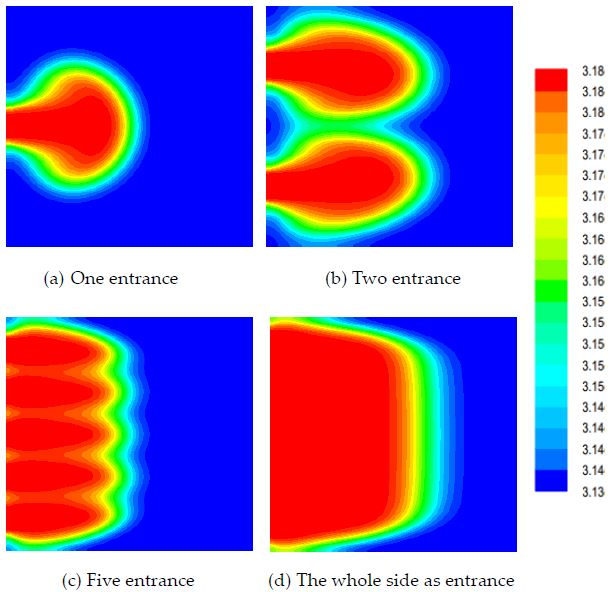
\includegraphics[width=12cm]{fig24.jpg}
\caption{The simulation results of different ways of arranging entrances} \label{fig24}
\end{figure}

From the above figure, the more the entrances are, the evener the temperature will be. Recalling on the before simulation outcome, when there is only one entrance for inflow, the temperature of corners is quietly lower than the middle area.

In conclusion, if we design more entrances, it will be easier to realize the goal to keep temperature even throughout the bathtub.

\item Model Application

Our before discussion is based on ideal assumptions. In reality, we have to make some corrections and improvement.

\begin{itemize}
\item[1)] Adding hot water continually with the mass flow of 0.16 kg/s. This way can ensure even mean temperature throughout the bathtub and waste less water.

\item[2)] The manufacturers can design an intelligent control system to monitor the temperature so that users can get more enjoyable bath experience.

\item[3)] We recommend users to add bubble additives to slow down the water being cooler and help cleanse. The additives with lower thermal conductivity are optimal.

\item[4)] The study method of our establishing model can be applied in other area relative to convection heat transfer, such as air conditioners.
\end{itemize}
\end{itemize}